\def\year{2017}\relax
%File: formatting-instruction.tex
\documentclass[letterpaper]{article} %DO NOT CHANGE THIS
\usepackage{aaai17}  %Required
\usepackage{times}  %Required
\usepackage{helvet}  %Required
\usepackage{courier}  %Required
\usepackage{url}  %Required
\usepackage{graphicx}  %Required
\frenchspacing  %Required
\setlength{\pdfpagewidth}{8.5in}  %Required
\setlength{\pdfpageheight}{11in}  %Required
%PDF Info Is Required:
  \pdfinfo{
/Title (Detecting Emergency Situations by Inferring Locations in Twitter)
/Author (Hernan Sarmiento, Jaime Campos, Barbara Poblete)}
\setcounter{secnumdepth}{0}  
 \begin{document}
% The file aaai.sty is the style file for AAAI Press 
% proceedings, working notes, and technical reports.
%
\title{Detecting Emergency Situations by Inferring Locations in Twitter}
\author{Hern\'an Sarmiento\\ Department of Computer Science \\ University of Chile, Santiago, Chile \\ hsarmien@dcc.uchile.cl
	\And Jaime Campos \\ Department of Geophysics \\ University of Chile, Santiago, Chile \\ jaime@dgf.uchile.cl
	\And B\'arbara Poblete\\ Department of Computer Science \\ University of Chile, Santiago, Chile \\ bpoblete@dcc.uchile.cl
}

\maketitle
\begin{abstract}
Most methods to detect emergency situations using Twitter rely on keyword. The problem of keyword-based methods is the need to train in specific domains for different type of events, for example: earthquakes, typhoons, terrorist attacks, tornadeos, etc.
Our proposal is to rather use the recurring mention of a country-locations in microblogging messages to identify such events without using keywords and characterize through of inter-arrival times the urgency of situation.
\end{abstract}

\noindent
\section{Introduction}

Social media has become a major channel for communication during high-impact real events, for example: elections, sports events, emergency situations, etc. In any event, users act as social sensors where they share and post their mood, opinions, photos, videos and exact location by GPS in only $8\%$ of messages.

Microblogging has played a critical role during emergency situations because traditional media have damage to infrastructure and affected people can not express their current status. For this reason, researchers have studied the behaviour during these events for to detect, summarize and classifyng messages with the goal to help authorities and the general public with situational awareness.

In current works \cite{kumar2011};\cite{ashktorab2014tweedr};\cite{imranaidr2014}, these tasks are solved with methods rely on keywords over Twitter public streaming API. The problem with these keyword-based methods is the need to train in specific domains for different type of events.\cite{olteanu2014} generate set of keywords with different datasets but sometimes arise specific terms for one event, for example \textit{\#eqnz} for Earthquake in New Zealand or \textit{\#pabloph} for Typhoon Pablo in Philippines.

We propose a method based on recurring mention of country-locations in messages' metadata for detecting a new emergency situation without using set of keywords related to crisis situation. These mentions can to occur into the text message, the GPS coordinates, the location of the user profile or the combination of these features.


\section{Methodology}

We collect random messages without using keyword or bounding box for 3 days - before, during and after event - for Mw 6.9 chilean Earthquake (April 24, 2017 21:38:28 UTC) using Twitter public streaming API. Addionality, we extract locations for Chile from GeoNames database with at least 5000 person per location. We create 4 signals associated with country-locations in the Tweet's metadata. To do this, we inspect the text of the message, the GPS coordinates and the location of the user profile, seeking any mention of country-locations into text (See Table \ref{signalsTweets} for number of tweets by signal):

\begin{itemize}
	\item \textit{Countrytxt}: text tweet contains a location associated with Chile.
	\item \textit{Countryusr}: user who shares a message has profile with location associated with Chile.
	\item \textit{Countrygeo}: tweet contains GPS coordinates in Chile.
	\item \textit{Countrytxt-usr}: user shares a message that contains a location associated with Chile and his profile as well.
\end{itemize}

\begin{table}[]
	\centering
	\begin{tabular}{|l|l|}
		\hline
		Total Tweet    & 13,655,428 \\ \hline
		Countrytxt     & 66,996     \\ \hline
		Countryusr     & 47,818     \\ \hline
		Countrygeo     & 1,161      \\ \hline
		Countrytxt-usr & 3,519      \\ \hline
	\end{tabular}
	\caption{Number of Tweets by Signal}
	\label{signalsTweets}
\end{table}

For each signal, we consider original tweets and retweets, compute their frequency per minute and normalize respect to the maximum value of each (Figure 1).

\begin{figure}[h]
	
	\centering
	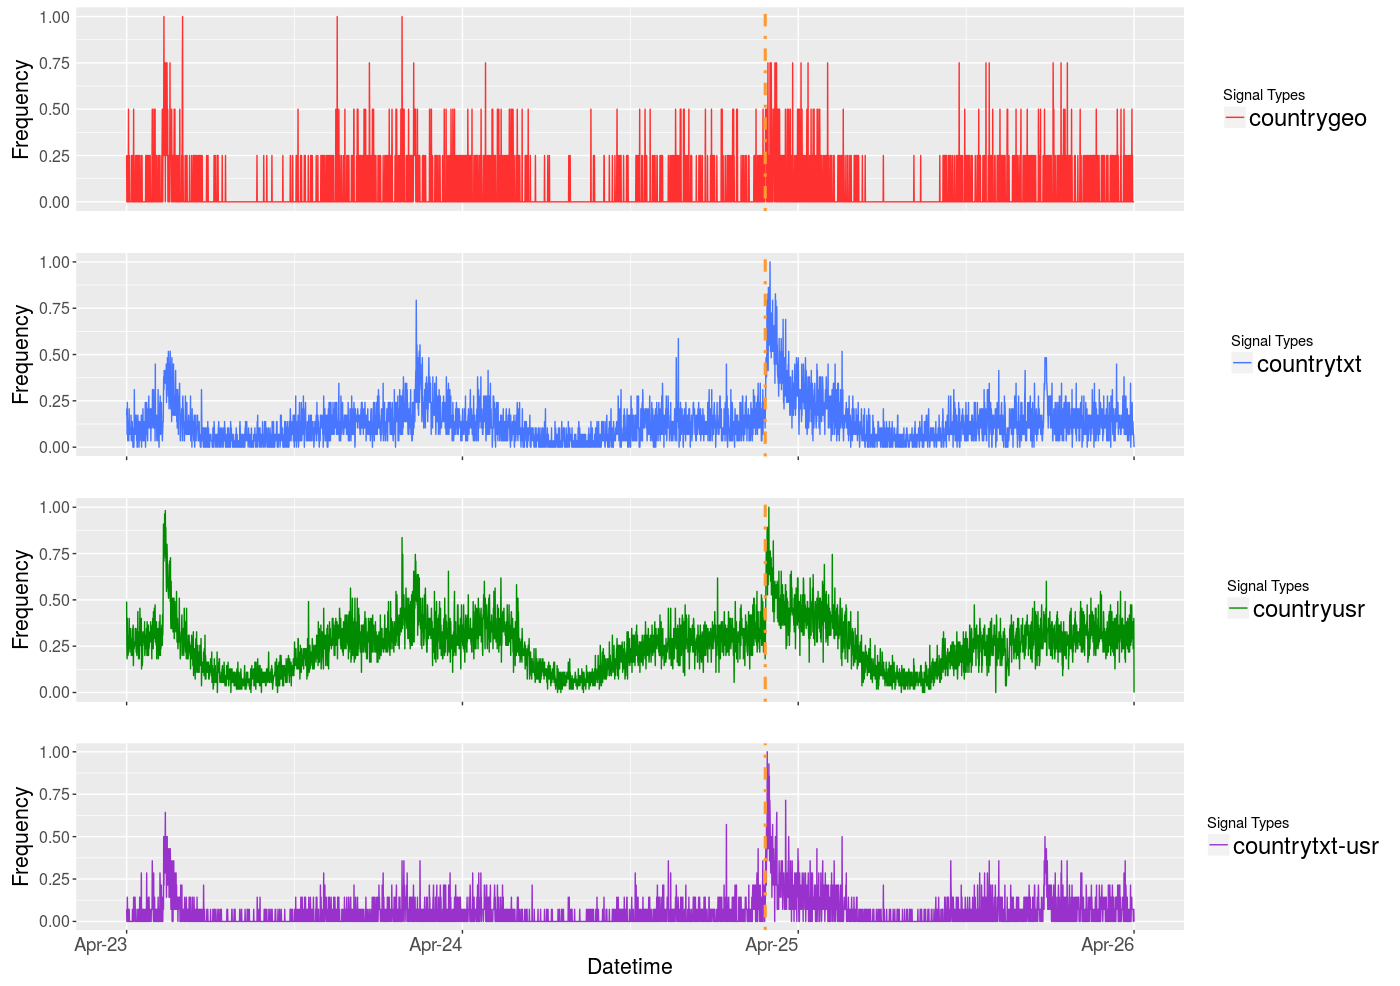
\includegraphics[width=0.5\textwidth]{freq_per_minute.png}
	\caption{Normalized Frequency per Minute for Mw 6.9 chilean Earthquake}
\end{figure}

\section{Results and Discussion}

We compare signals when the earthquake occur. In all cases, signals detect a new emergency situation except the \textit{countrygeo} signal having lower frequency but represent the exact location where from message was sent . This result can be explained because a little portion of users use GPS coordinates when shares a message (near to $8\%$ or least). The other signals detect correctly a new emergency situation because its maximum values coincide with earthquake's datetime.

However, the signals that represent country-locations into the text message or the location of the user profile, exhibit noise that can generate burst for other event types. Sometimes, these signals have a relative behaviour that depends on the average daily user's activity of country. 

For reducing this noise exhibited by independent features, we combine the \textit{countrytxt} and the \textit{countryusr} signals for generating the \textit{countrytxt-usr} signal. This means that a user with an inferred locality of Chile, shares a message that contains an inferred locality of Chile into the text tweet. Moreover, we can consider that user (probably in Chile) shares information of Chile in his message, thus, the user cares about things that happen in Chile.

\subsection{Characterization of the Signals}

We characterize an emergency situation by using \textit{inter-arrival times} between consecutive social media messages within a sub-time series. The inter-arrival time is defined as $d_{i} = t_{i+1} - t_{i}$ where $d_{i}$ denotes the difference between two consecutive social media messages $i$ and $i+1$ that arrived in moments $t_{i}$ and $t_{i+1}$, respectively.

Using the \textit{countrytxt-usr} signal, which detect a new emergency situation and has less noise than other signals, we characterize and compare two different sub-time series within of the event. For these tasks, we extract messages 1 hour before earthquake and messages 10 minutes after earthquake (Figure \ref{interarrival}). 
\begin{figure}[h]
	\centering
	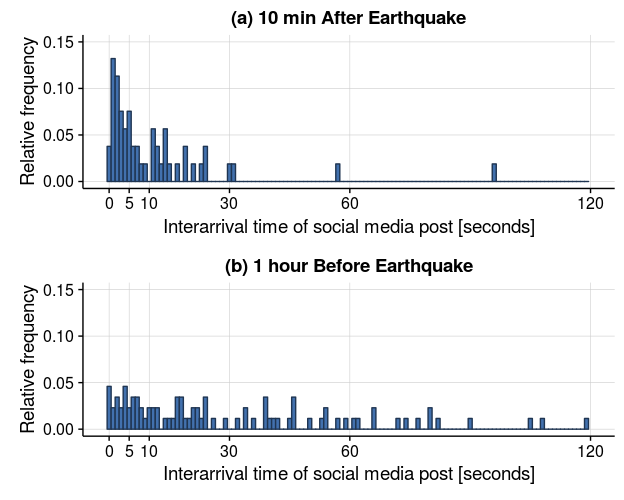
\includegraphics[width=\columnwidth]{interarrival.png}
	\caption{Inter-arrival Time Before and During Mw 6.9 chilean Earthquake}
	\label{interarrival}
\end{figure}

On the one hand, when an unpredicted emergency situation occur, the urgency of messages can be represented on the first bins, where at least $60\%$ of the messages have an inter-arrival time $d_{i} < 10$ seconds (Figure \ref{interarrival}.a). Therefore, we learn that many users in the same country, share messages named their current location in the country almost simultaneously.

On the other hand, considering a sub-time series before to earthquake, bins are spreaded and $28\%$ of the messages have an inter-arrival time $d_{i} < 10$ seconds (Figure \ref{interarrival}.b). Thus, users in the same country are not simultaneously affected by the same spatio-temporal event, do not share their current location in the message.

\section{Conclusion and Future Work}
Detect a emergency situation without using a specific-domain of keywords is important because training data is hard work for researchers. We presented a proposal for detecting this event type using only locations asociated to the country. These locations, unlike keywords, do not change over time and do not emerge spontaneously during a emergency situation.

In the future, we will investigate other emergency situations but with local impact in the first phase after event, e.g. terrorist attack, plane crash, etc.
 
\bibliographystyle{aaai}
\bibliography{bio}




\end{document}
